\begin{frame}
    \begin{itemize}
        \item Liquid photopolymers (photosensitive)
        \item Printed object is pulled out of the material from bottom to top
        \item Each layer is partially cured by \acs{uv} light projector
        \item Higher precision than with \acs{fff} is possible
        \item Prices are also decreasing (inexpensive printers $\approx$ \SI{250}{\sieuro})
    \end{itemize}
\end{frame}

\begin{frame}
    \begin{figure}
        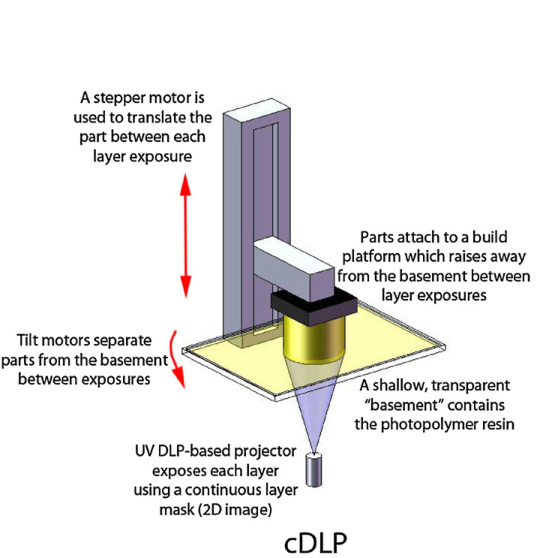
\includegraphics[height=7cm]{rapid-prototyping/digital-light-processing.pdf}
        \caption{\glsentrydesc{dlp}}
    \end{figure}
\end{frame}